\documentclass[a4paper,final]{article}
\usepackage{subfig}
\usepackage[dutch]{babel}
\usepackage{minutes}
\usepackage{graphicx}
\usepackage{epstopdf}
\usepackage{float}

\title{Notulen 016 overleg team 33}
\author{Guus}
\minutesstyle{header=table, vote=list, contents=true, columns={1}}

\begin{document}
%\selectlanguage{dutch}

\begin{Minutes}{Overleg 014 team 33}
\participant{Bernard van Gastel, Guus Bonnema, Stefan Versluys, Jeroen Kleijn}
\subtitle{Project toelichting en architectuur}
\minutetaker{Guus}
\minutesdate{29 november 2014}
\location{Skype}

\maketitle% This is where LaTeX makes the title

\newcommand{\w}[1]{\textsc{#1}}

\topic{Correcties vorige notulen} Bernard werkt formeel bij de OU. In zijn
project werkt hij samen met mensen van de RU en anderen.

\topic{Huidige en gewenste architectuur}

\begin{center}
	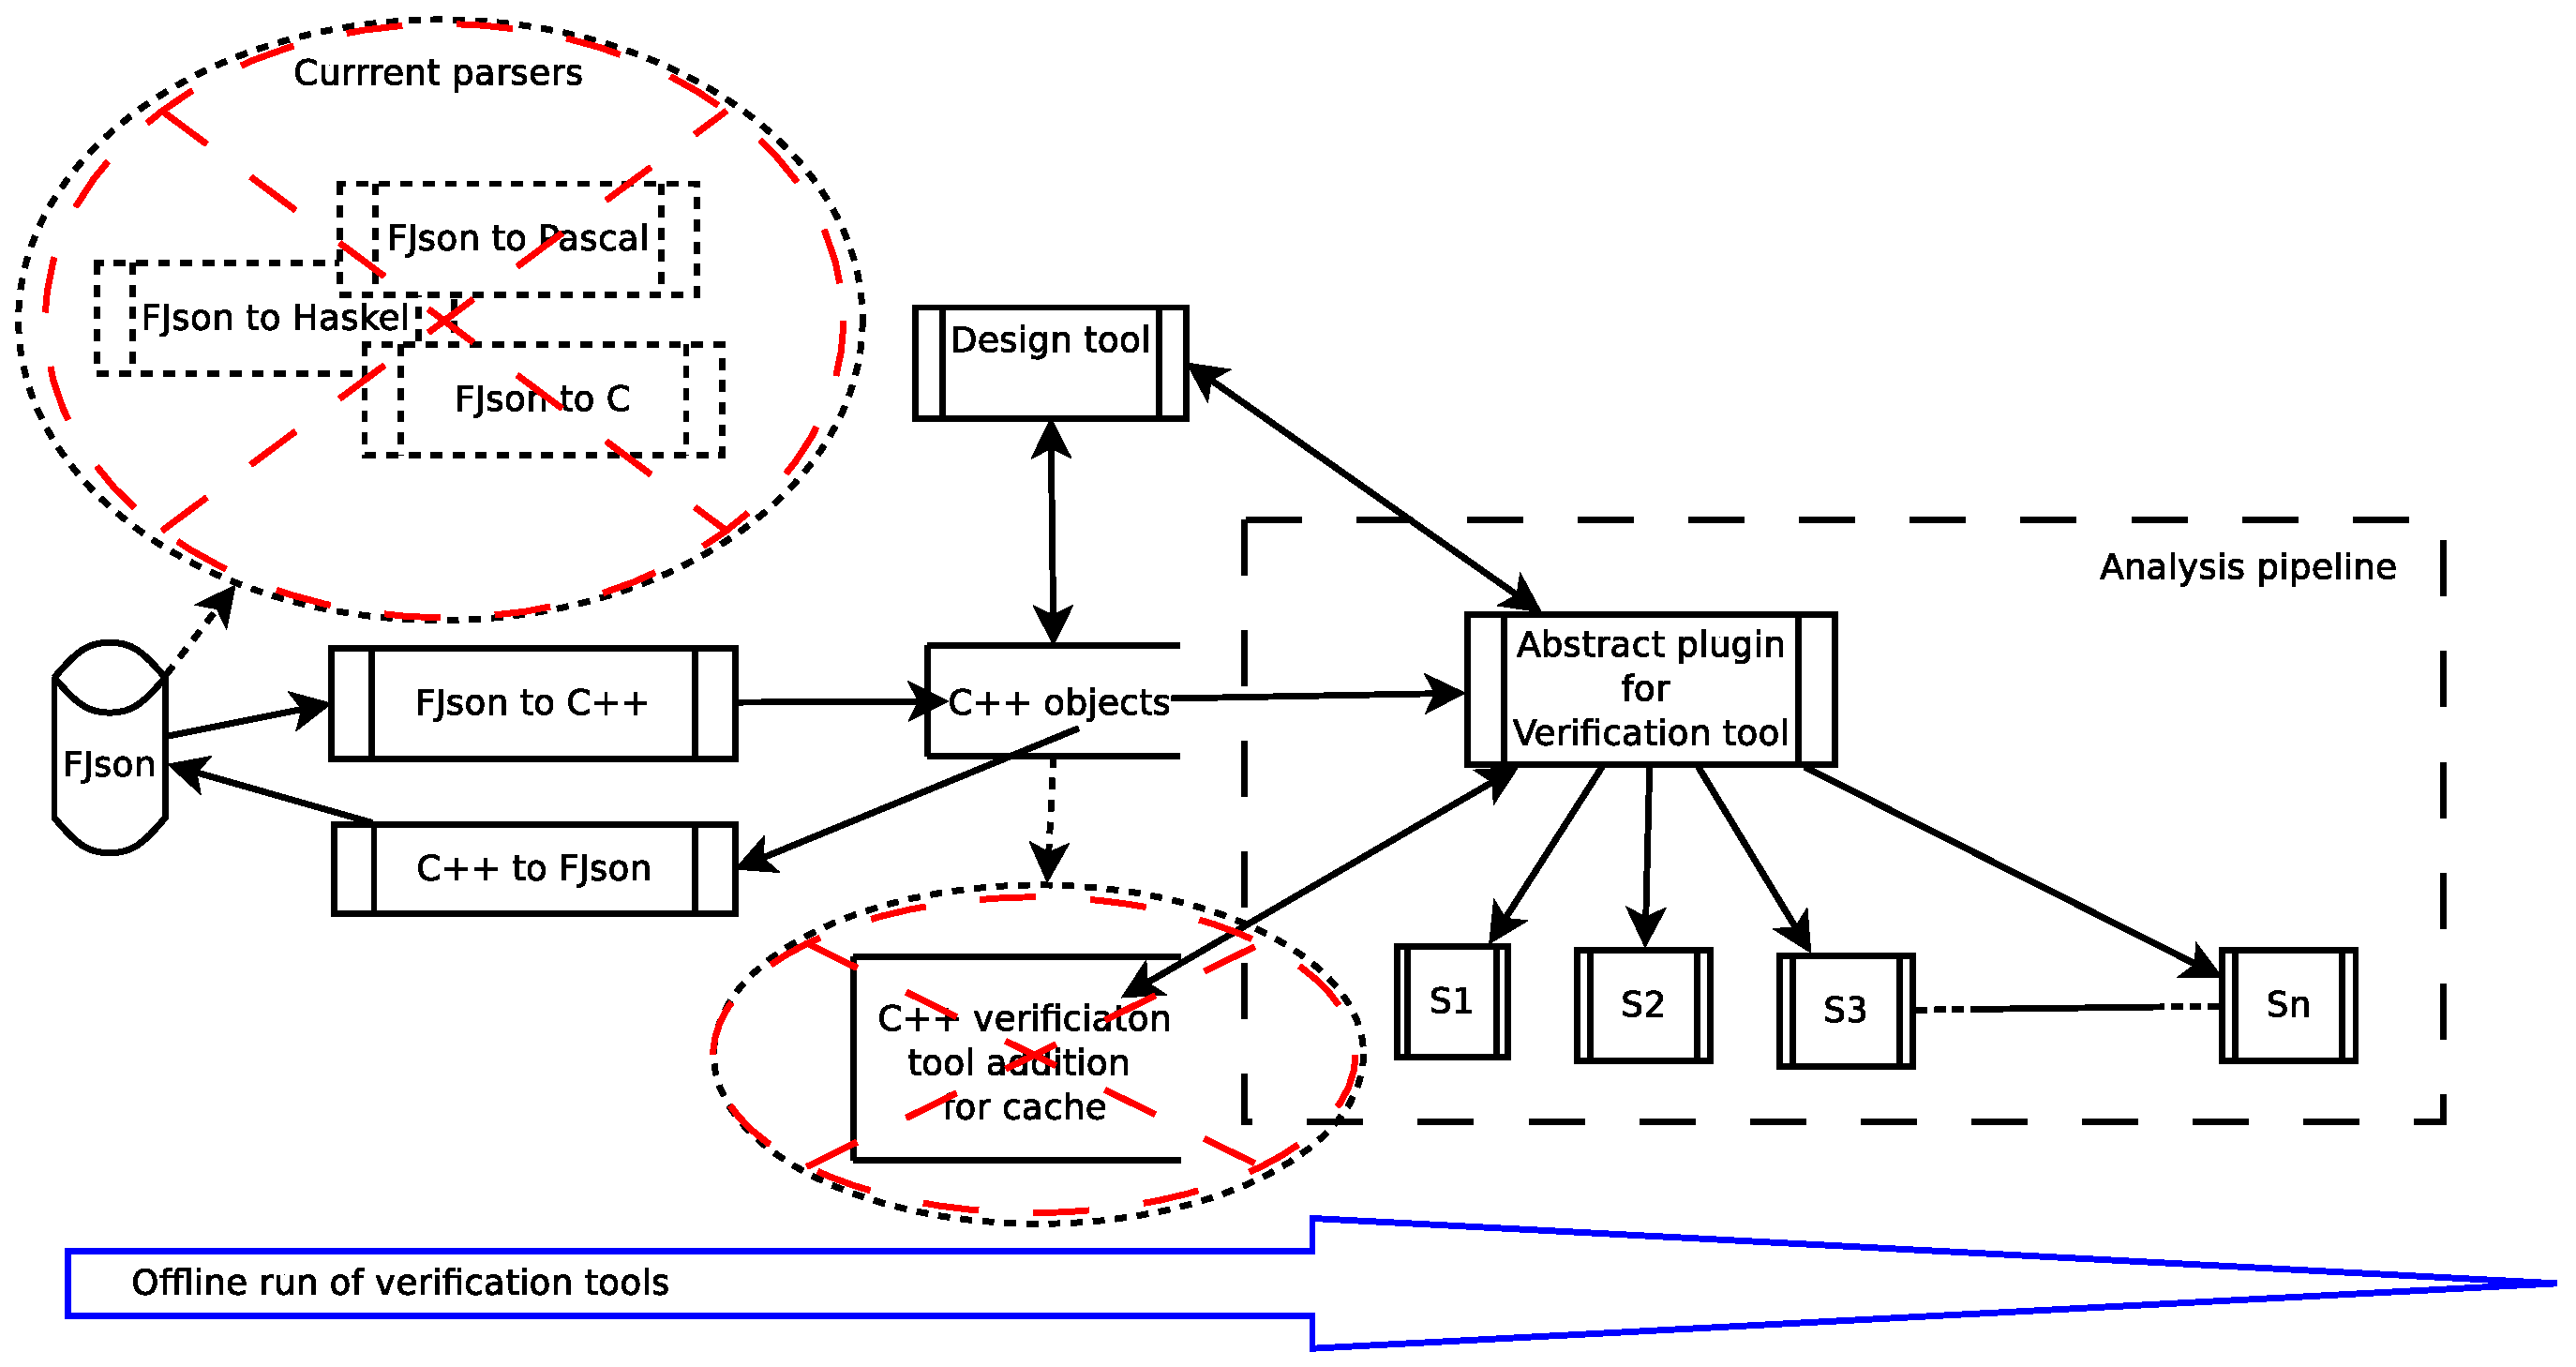
\includegraphics[width=.9\linewidth]{2014-11-29-meeting-architecture-tool-1.eps}
	\captionof{figure}{High level architecture for GUI and pipeline (eerste versie)}
	\label{fig:architecture-high-level-1}
\end{center}

\begin{center}
	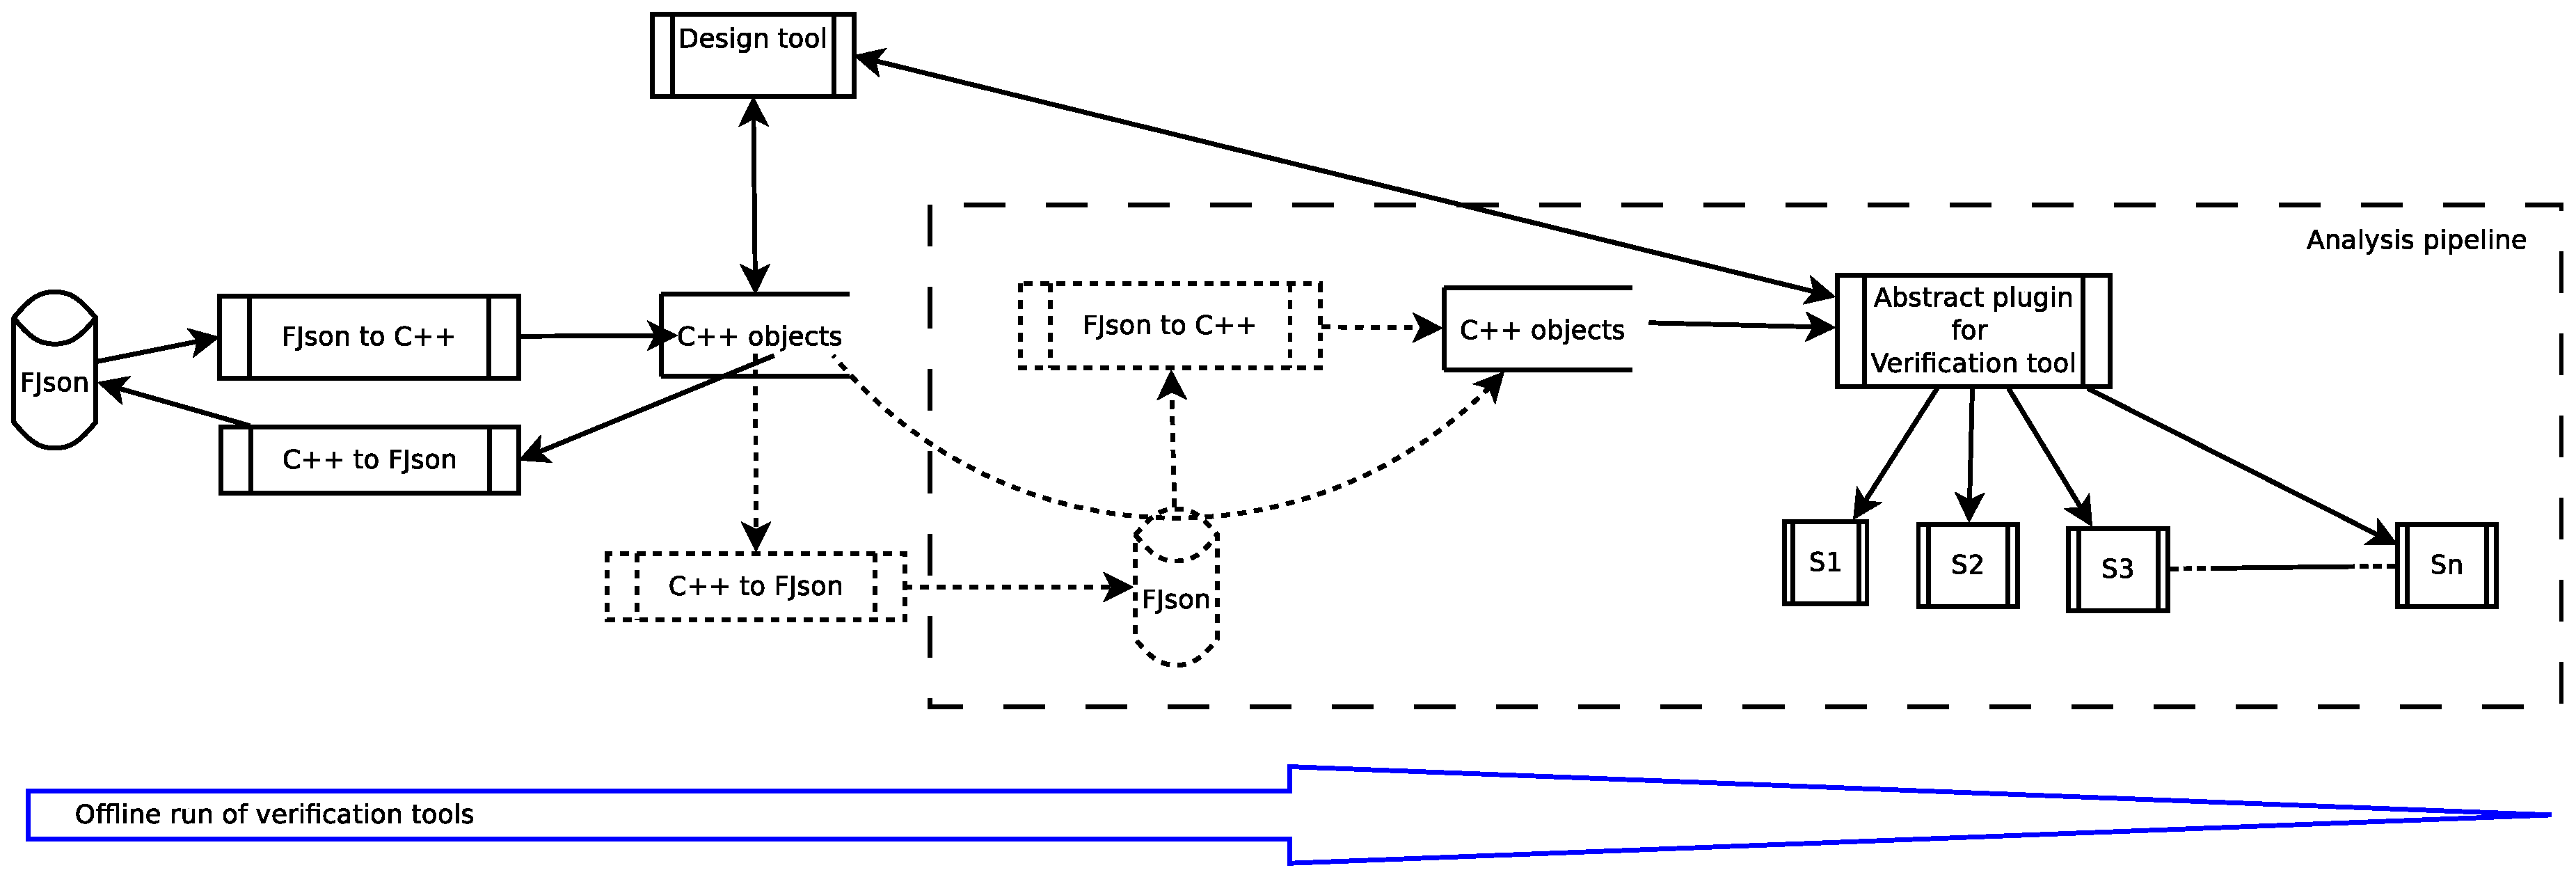
\includegraphics[width=.9\linewidth]{2014-11-29-meeting-architecture-tool-2.eps}
	\captionof{figure}{High level architecture for GUI and pipeline (tweede versie)}
	\label{fig:architecture-high-level-2}
\end{center}

\begin{description} 

	\item[Offline run van verificatie] Vanaf de command line of vanuit een
		script kunnen de onderzoekers alle verificitie tools draaien over een
		model om de uitvoer via logfiles te verzamelen dan wel op standaard
		output te krijgen. Deze batch run is noodzakelijk bij het
		verifi\"{e}ren van grotere modellen. Men voert dit ook wel 's nachts
		uit.

	\item[Online run van verificatie] Bij het gebruik van het online design
		tool moet men selectief verificatie tools kunnen kiezen.  De in te
		vullen parameters hangen direct samen met de geselecteerde tools.
		
	\item[plugin architectuur] De plugin architectuur is iets dat de
		verificatie stappen uitvoert voor 1 of meer verificatie tools. De
		werking en samenhang van de verificatie tools zelf is buiten scope. De
		plugin architectuur en de generieke plugin code is in scope. Het doel
		van de plugin is de hoeveelheid boilerplate code te minimaliseren en
		het gemak van introduceren van een nieuw tool te maximalieren.

	\item[Plugin communicatie] De communicatie tussen plugin en ontwerp tool is
		onderwerp van discussie. De ideeen zijn gebruik te maken van pipes of
		van zeroMQ. Het voordeel van zeroMQ is platform onafhankelijkheid
		terwijl zeroMQ ook gebruik maakt van pipes als de processen op dezelfde
		machine draaien.

	\item[Plugin implementatie]	Daarnaast is de communicatie afhankelijk van de
		implementatie. Bij implementatie binnen een proces kan de design tool
		het geheugen delen. Bij implementatie in een ander proces is dat niet
		zeker (open punt). Bij implementatie op een andere machine kan dat
		zeker niet\footnote{Voor de volledigheid genoemd: het is geen onderwerp
		binnen dit project}.

	\item[Composite object] Er zijn twee vormen van composite objects. De
		eerste is een NoC en kan de onderzoeker in composite vorm op dezelfde
		manier gebruiken als een primitive object. De tweede is een
		geparametriseerde composite object. Daar is de composite een template
		waaruit de onderzoeker een daadwerkelijk NoC genereert. 

		Als voorbeeld geldt een matrix van $n \times n$ objecten, waarbij $n$
		variabel is. Tijdens het bekijken van de NoC zal deze composite in haar
		template vorm te zien zijn. Bij het uitwerken van de totale netwerk
		structuur genereert het systeem de werkelijke instantie van de
		composite, dus in dit geval een $n \times n$ matrix van objecten.

		Bernard refereert aan deze composites als ``recursief''. Dit onderwerp
		is nog ter discussie. Het genereert een nieuw requirement, dat Bernard
		voor ons project op ``should have'' prioriteit zet. Dat betekent dat
		het niet per se binnen ons project implementatie vindt, maar dat het
		wel in een volgend project te implementeren moet zijn.

		Ter indicatie van de complexiteit gaf Bernard aan dat dit de reden was
		voor het ontstaan van het huidig project: het vorige systeem kon de
		wijziging structureel niet goed opnemen, het was te complex.
		
	\item[Current parsers] Op dit moment zijn er meerdere parsers van FJson
		naar interne structuren. Het doel van Bernard is het aantal parsers tot
		\'e\'en te beperken: die van en naar een C++ structuur. Tevens is dit
		de enige datastructuur zodat verschillen in semantiek tot het verleden
		behoren.

	\item[C++ verification tool addition] De huidige C++ datastructuur bevat
		behalve gegevens voor het model ook gegevens voor de verificatie tools.
		Het doel is caching zodat verificatie minder lang duurt.  Het is ter
		discussie of deze gegevens in het C++ model thuishoren dan wel ergens
		anders bij de verificatie modules thuis horen.  

		Na discussie stelde Jeroen het zwakke punt aan de kaak: na compileren van
		de module dan is de structuur wellicht anders. Bovendien staat de cache
		dan niet meer in het geheugen en moet je het naar een file schrijven.
		Na deze discussie vindt Bernard de cache voor nu niet meer belangrijk.
		Als het voor een specifiek tool belangrijk wordt, dan kan de
		toolbouwer dit in zijn deel van het tool inbouwen. Het design tool
		bemoeit zich hier dan niet mee.

	\item[Additionele libraries] Voor process control en thread control moeten
		we i.v.m. platform onafhankelijkheid leunen op tools die threads en
		processen platform onafhankelijk kunnen aansturen. De ideeen gaan uit
		naar de library \w{Boost}. Zie opmerking in volgend topic over code van
		Bernard uit \w{Boost}

\end{description}

\topic{Diverse onderwerpen}

\subtopic{Boost} Over het gebruik van \w{Boost} waarschuwt Bernard dat deze
onder apple alleen in zijn geheel te installeren is. Als ik het goed heb
begrepen moeten alle \w{Boost} libraries vanuit source gecompileerd worden: dat
duurt lang.  Voor Linux en Windows is dit probleem er niet. Bernard heeft voor
een ander project code uit \w{Boost} ge\"{i}soleerd, dat wij kunnen gebruiken.

\subtopic{0mq} Over \w{zeroMQ} is Bernard gematigd terughoudend. De library
heeft een goede reputatie, maar de voordelen voor ons project zijn beperkt tot
platform onafhankelijkheid.  Omdat platform onafhankelijkheid wel erg
belangrijk is en gebruik van \w{0MQ} geen merkbare nadelen heeft, lijkt dit een
goede keuze.

Bernard meent dat dit wellicht ook zonder \w{zeroMQ} goed op te lossen is. Open
punt, ter discussie.

\subtopic{Use cases met delen informatie} Naar aanleiding van de mail van Guus
over use cases waar een docent een model toont aan studenten of een onderzoeker
een model wil delen, maakt definitief geen onderdeel uit van het ontwerp tool.

De nadere toelichting is dat het tool een research tool blijft en geen
professionele aspiraties heeft. Delen van de gegevensstructuren via de
applicatie hoort niet bij de doelstellingen voor dit project.

\topic{Open punten}

\begin{description} 
	
	\item[Boost] Is \w{Boost} nodig? Is het nuttig?

	\item[0MQ] Is \w{zeroMQ} nodig? Is het nuttig?

	\item[Implementatie plugin] Gaan we de plugin in hetzelfde proces opnemen
		als thread of gaan we het als apart proces laten draaien? 

	\item[Communicatie plugin] Gaan we gebruik maken van \w{zeroMQ} voor
		communicatie met plugin en/of componenten?

	\item[Communicatie plugin] Gaan we gebruik maken van boost voor thread of
		proces management?

	\item[Parameteriseren van composites] Hoe gaan we parameterisering opnemen
		in onze architectuur?

	\item[Parameteriseren van composites] Gaan we parameterisering
		implementeren in dit project?

\end{description}

\end{Minutes}
\end{document}
